%; whizzy section -pdf xpdf -latex ./whizzypdfptex.sh
% latex beamer presentation.
% platex, latex-beamer でコンパイルすることを想定。 

%     Tokyo Debian Meeting resources
%     Copyright (C) 2008 Junichi Uekawa

%     This program is free software; you can redistribute it and/or modify
%     it under the terms of the GNU General Public License as published by
%     the Free Software Foundation; either version 2 of the License, or
%     (at your option) any later version.

%     This program is distributed in the hope that it will be useful,
%     but WITHOUT ANY WARRANTY; without even the implied warranty of
%     MERCHANTABILITY or FITNESS FOR A PARTICULAR PURPOSE.  See the
%     GNU General Public License for more details.

%     You should have received a copy of the GNU General Public License
%     along with this program; if not, write to the Free Software
%     Foundation, Inc., 51 Franklin St, Fifth Floor, Boston, MA  02110-1301 USA

\documentclass[cjk,dvipdfmx,12pt]{beamer}
\usetheme{Tokyo}
\usepackage{ulem}
\usepackage{tabularx}

\usepackage{fancybox}
\usepackage{fancyvrb}   
\usepackage{float}

% commandline環境を定義。画面入出力についてはcommandline環境
% で表記する
\newenvironment{commandline}%
{\VerbatimEnvironment
  \begin{Sbox}\begin{minipage}{0.9\hsize}\begin{fontsize}{7.3}{7.3} \begin{BVerbatim}}%
{\end{BVerbatim}\end{fontsize}\end{minipage}\end{Sbox}
  \setlength{\fboxsep}{8pt}
% start on a new paragraph

\vspace{6pt}% skip before
\fcolorbox{dancerdarkblue}{dancerlightblue}{\TheSbox}

\vspace{6pt}% skip after
}
%end of commandline

\definecolor{dancerdarkblue}{rgb}{0,0.08,0.45}
\definecolor{dancernormalblue}{rgb}{0.8,0.9,0.95}
\definecolor{dancerlightblue}{rgb}{0.8,0.95,1}


%  preview (shell-command (concat "evince " (replace-regexp-in-string "tex$" "pdf"(buffer-file-name)) "&"))
%  presentation (shell-command (concat "xpdf -fullscreen " (replace-regexp-in-string "tex$" "pdf"(buffer-file-name)) "&"))

%http://www.naney.org/diki/dk/hyperref.html
%日本語EUC系環境の時
\AtBeginDvi{\special{pdf:tounicode EUC-UCS2}}
%シフトJIS系環境の時
%\AtBeginDvi{\special{pdf:tounicode 90ms-RKSJ-UCS2}}

\title{東京エリア Debian 勉強会}
\subtitle{資料}
\author{上川 純一 dancer@debian.org\\IRC nick: dancerj}
\date{2008年3月15日}
\logo{
\includegraphics[width=8cm]{image200607/openlogo-light.eps}}


% 間のタイトルページ用
\newcommand{\emtext}[1]{
\begin{frame}{}
 
\begin{minipage}{0.55\hsize}
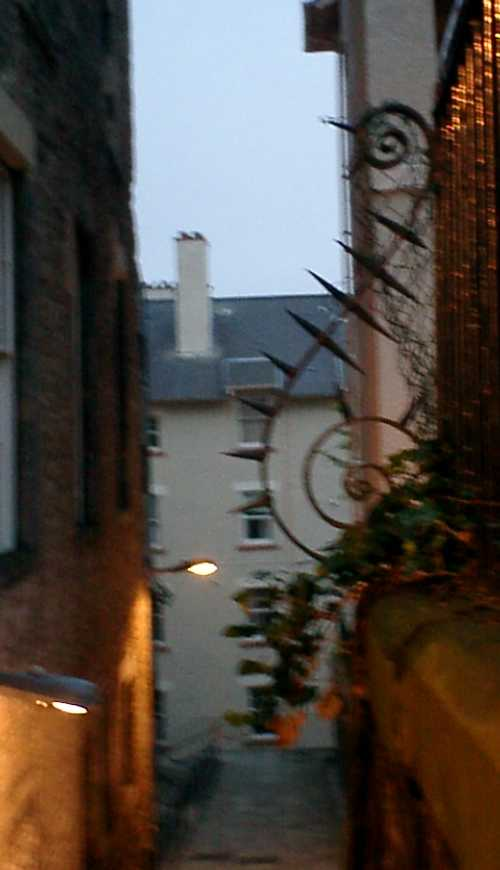
\includegraphics[width=1\hsize]{image200707/gurutitle.jpg}
\end{minipage}
\begin{minipage}{0.39\hsize}
 {\Huge #1
 }
\end{minipage}
\end{frame}
}

% 三択問題用
\newcounter{santakucounter}
\newcommand{\santaku}[5]{%
\addtocounter{santakucounter}{1}
\frame{\frametitle{問題\arabic{santakucounter}. #1}
%問題\arabic{santakucounter}. #1
\begin{minipage}[t]{0.8\hsize}
 \begin{itemize}
 \item
      \begin{minipage}{0.2\hsize}
      
\includegraphics[width=0.9\hsize]{image200703/janken-A.png}\end{minipage} 
       \begin{minipage}{0.6\hsize}
       A #2\end{minipage}\\
 \item
      \begin{minipage}{0.2\hsize}
      
\includegraphics[width=0.9\hsize]{image200703/janken-B.png}\end{minipage} 
       \begin{minipage}{0.6\hsize}
       B #3\end{minipage}\\
 \item
      \begin{minipage}{0.2\hsize}
      
\includegraphics[width=0.9\hsize]{image200703/janken-C.png}\end{minipage} 
       \begin{minipage}{0.6\hsize}
       C #4\end{minipage}\\
 \end{itemize}
\end{minipage}
}
\frame{\frametitle{問題\arabic{santakucounter}. #1}
%問題\arabic{santakucounter}. #1
\begin{minipage}[t]{0.8\hsize}
\begin{itemize}
 \item
      \begin{minipage}{0.2\hsize}
      
\includegraphics[width=0.9\hsize]{image200703/janken-A.png}\end{minipage} 
       \begin{minipage}{0.6\hsize}
       A #2\end{minipage}\\
 \item
      \begin{minipage}{0.2\hsize}
      
\includegraphics[width=0.9\hsize]{image200703/janken-B.png}\end{minipage} 
       \begin{minipage}{0.6\hsize}
       B #3\end{minipage}\\
 \item
      \begin{minipage}{0.2\hsize}
      
\includegraphics[width=0.9\hsize]{image200703/janken-C.png}\end{minipage} 
       \begin{minipage}{0.6\hsize}
       C #4\end{minipage}\\
\end{itemize}
\end{minipage}
\begin{minipage}[t]{0.15\hsize}
答えは:

\vspace{1cm}

  {\huge \hspace{1cm}#5}
  \hspace{-6cm}\includegraphics[width=4cm]{image200703/janken-#5.png}
 \end{minipage}}
}

\begin{document}

\frame{\titlepage{}}


\section{Intro}

\emtext{設営準備にご協力ください}

\begin{frame}{会場までの道のり}
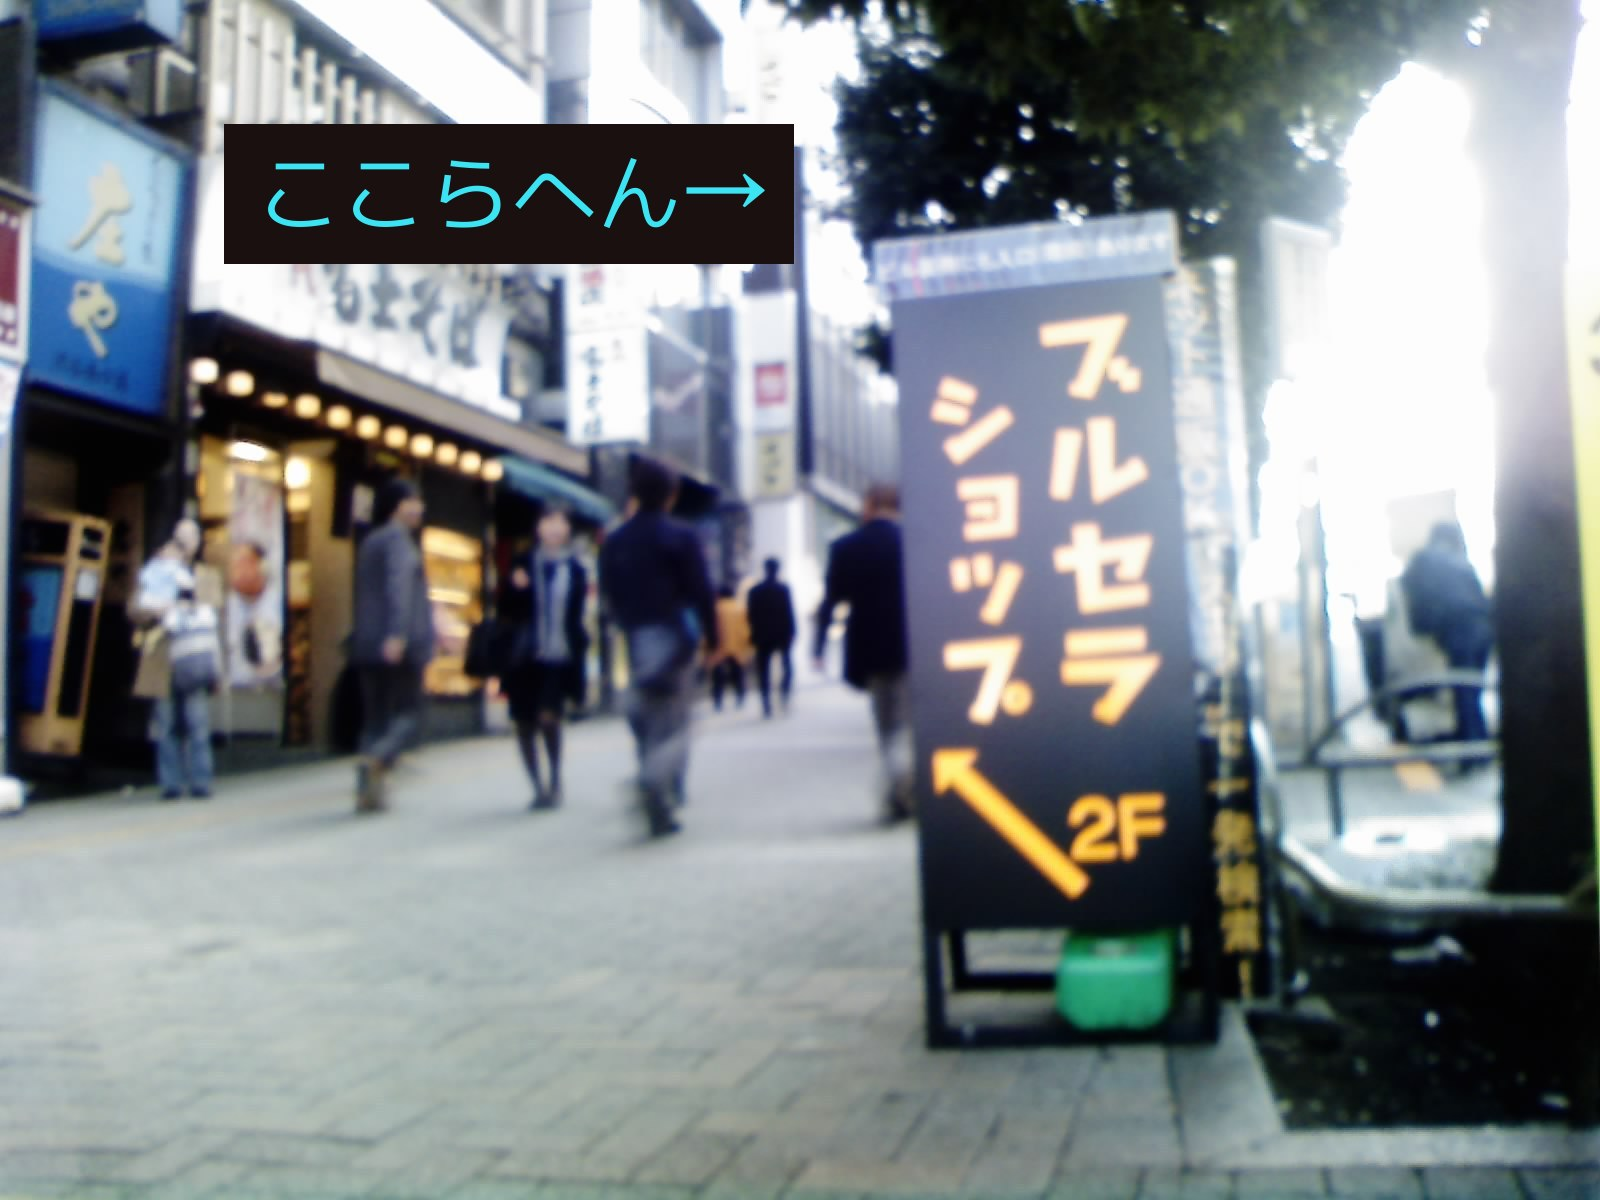
\includegraphics[width=1\hsize]{image200803/google-entry.jpg}
\end{frame}

\begin{frame}
 \frametitle{Agenda}
\begin{minipage}[t]{0.45\hsize}
  \begin{itemize}
  \item 注意事項
	\begin{itemize}
	 \item 撮影禁止
	 \item この部屋で話されたことはこの部屋の外には一歩も出ません
	 \item 無線LANは ESSID google-guest
	\end{itemize}
  \item quiz
  \item 最近のDebian関連のイベント
	\begin{itemize}
	 \item 前々回
	 \item 前回 (OSC)
	\end{itemize}
 \end{itemize}
\end{minipage} 
\begin{minipage}[t]{0.45\hsize}
 \begin{itemize}
  \item データだけのDebianパッケージ
  \item Debianでのライセンスの考え方
 \end{itemize}
\end{minipage}
\end{frame}

\section{最近}

\begin{frame}
 \frametitle{前々回のAgenda}
\begin{minipage}[t]{0.45\hsize}
  \begin{itemize}
  \item 注意事項
	\begin{itemize}
	 \item 飲食禁止
	 \item 政治/宗教/営利活動禁止
	\end{itemize}
  \item quiz
  \item 最近のDebian関連のイベント
	\begin{itemize}
	 \item 前回
	\end{itemize}
 \end{itemize}
\end{minipage} 
\begin{minipage}[t]{0.45\hsize}
 \begin{itemize}
  \item 2008年度 Debian 勉強会企画
  \item Debian Package 管理の流れ
 \end{itemize}
\end{minipage}
\end{frame}


\begin{frame}{Git 特集}

Debian勉強会のリポジトリはGit管理です。
Gitの使い方がわからないといっている方々、よんでおいてください。


\includegraphics[width=0.4\hsize]{image200803/gihyo200804.jpg}

\end{frame}


\section{Debian勉強会とは}
\emtext{Debian勉強会とは}
\begin{frame}{Debian勉強会とは}
語ってみる。
\end{frame}


\section{DWN quiz}
\begin{frame}{Debian 常識クイズ}

Debian の常識、もちろん知ってますよね?
知らないなんて恥ずかしくて、知らないとは言えないあんなことやこんなこと、
みんなで確認してみましょう。

今回の出題範囲は、\url{http://lists.debian.org/debian-devel-announce/} にある最近の
アナウンス文書です。

\end{frame}

\subsection{問題}

%問題をコピペ

 \santaku
 {lennyでのリリースゴールの1つにGCC 4.3でのビルドが通ることが挙げられているが、
 それに伴って変更する必要が最も多く生じるのは、どの言語で書かれたプログラムか?}
 {C}
 {C++}
 {Ruby}
 {B}
 
 \santaku
 {今のところlennyで完全に削除される予定なのは次のうちどれか?}
 {GNOME 1.x}
 {KDE 3.x}
 {Linux 2.x}
 {A}
 
 \santaku
 {Debianに宣伝力がないと感じたDebianプロジェクトリーダー (DPL) のSam Hocevarが提案したのは?}
 {イベント会場でDebianロゴの入ったシャツを着て練り歩くDebian Tank Top \& Brief Team}
 {ロゴやTシャツのデザインなどマーケティング面の任務を一手に引き受けるDebian Marketing Team}
 {Debianのマスコットキャラクター「でびにゃん」}
 {B}
 
 \santaku
 {3月頭の時点でlennyのリリースにとって致命的なバグ (RCバグ) は460ほどあるが、
 それを減らす方法として推奨されているのは?}
 {debian/changelogに「closes: \#xxxxxx」と書いて片っ端からパッケージをアップロードする}
 {バグ退治パーティー (BSP) を開いて片っ端からパッケージを非メンテナアップロード (NMU) する}
 {RCバグを放置しているパッケージメンテナを片っ端から呼び出して説教する}
 {B}
 
 \santaku
 {lennyはリリースされると何になる?}
 {Debian 4.1}
 {Debian 5.0}
 {Ubuntu 8.0}
 {B}
 
 \santaku
 {lists.debian.orgの新しい検索エンジンには何が用いられているか?}
 {Google Search}
 {Hyper Estraier}
 {Xapian Omega}
 {C}
 
 \santaku
 {新しいarmelアーキテクチャに関する現況として適切でないものは?}
 {lennyのリリースアーキテクチャに含まれている}
 {全パッケージの90\%がビルドされている}
 {パッケージをftp.debian.orgからダウンロードできるようになっている}
 {A}
 
 \santaku
 {次の開発者のうち、今年のDPL選挙に立候補したのは?}
 {Lucas Nussbaum}
 {Junichi Uekawa}
 {Steve McIntyre}
 {C}

\section{最近の話題}

\emtext{OSC参加報告}

\section{事前課題紹介}
\emtext{事前課題の紹介}
% pre work home work

\begin{frame}{事前課題問題}

\begin{enumerate}
 \item データだけのパッケージでできること
 \item ソフトウェアのライセンスで不自由したこと
 \item 好きなソフトウェアライセンスとその理由
\end{enumerate}

\end{frame}

% (query-replace "\\subsection" "\\end{frame}\\begin{frame}")
% (query-replace "\\subsubsection" "\\textbf")

\begin{frame}{堀内寛己}

僕が好きなソフトウェアライセンスはGPLです。
理由は、ストールマンが好きだからです。

僕がストールマンのことを知ったのは、
20年以上前、東大の和田英一先生の講義をもぐって聞いたときのことです。
先生は、MITハッカーズの堕落と、
その中で孤軍奮闘しているストールマンの話をされました。
「でもストールマンは変わりませんねえ。
グニューって知ってますか? みんなタダなんですよ」
先生が英語の微妙なニュアンスを聞き分けられないわけがないので、
当時のストールマン自身が、freeの2つの意味を混同していたらしいことがわかります。
当然そのころ、GPLなんてありませんでした。
僕は幸い、入社まもなくGNU Emacsを使う幸運に恵まれ、
ストールマンへの敬意は確固たるものになり、
そのままGPLのことなど知らずにgcc-2のmakeをやったものです。
\end{frame}\begin{frame}{堀内寛己}
僕がGPLとその恐るべき意図について知ったのは、だいぶ後のことです。
Microsoftがこれをウィルス呼ばわりしたのほ、さらにその後のことです。
僕は、ウィルスという表現は、GPLについての最高の褒め言葉だと思っています。

\end{frame}\begin{frame}{山本ひろゆき}

「データだけのパッケージでできること」
インタープリタ依存のスクリプトパッケージなんかができますかね?今抱えてい
る ITP を片付けたら、kita2 (ruby スクリプト) を ITP しようかと迷っていま
す。パッケージング自体はできますが、ruby を知らないものでメンテナンスが
心配。誰か教えて!

「ソフトウェアのライセンスで不自由したこと」
某巨大掲示板発祥の開発プロジェクトあたりだと、有用なソフトウェアだが、ラ
イセンスは明記されていなく開発者も匿名で確認しようがないということもあり
ます。

「好きなソフトウェアライセンスとその理由」
GPL とか BSD ライセンスとか。DFSG 万歳!



\end{frame}\begin{frame}{Suguru Sekine}
「好きなソフトウェアライセンスとその理由」

[BSDライセンス]

 自由であり続けるために「自由でなければならない」という制約がない、
かつソースコードの公開を拒む自由があるためである。
私はソフトウェアは自由であるべきだと考えている。
また、自由であるための協力もできる限りの協力を行うつもりである。
しかし、自分が考えている事を他の人に強要したり、
または強要されたりすることがどうしても我慢できない。
以上のことから自由であることを強要されない点から
BSDライセンスをを評価しているという結論に至る。

\end{frame}\begin{frame}{Yamane Toshiaki}

「データだけのパッケージでできること」

データだけのパッケージというものが例えばフォントパケジ等を
指すという理解で文章を書いてみます。
できること、ではないかもしれませんが、自分が使いたいものを
選択する自由があると考えます。あるいは X と xfont なパッケージのように
アプリケーションとデータがそれぞれ互いに依存していない関係にする事が
できるのではないか、と考えます。データだけのパッケージと
そのデータを使うパッケージ間を疎結合な関係にしておくことによって、
保守とか拡張などの対応を柔軟に行なう事ができるのではないでしょうか。

\end{frame}\begin{frame}{沖中}

ライセンス的に配布が難しいデータは、自分でパッケージすることになると思いますが、
データだけのパッケージと言えばフォントが代表的だと思います。
辞書データもフリーの物が少ないので自分でパッケージ化できたら便利ですね。
それ以外の使い方としては、Webサイトのドキュメントをパッケージ化して
管理できないか考えています。そうなるとデータだけとはいきませんが、スクリプトだと
ビルド不要なのでデータと同じように扱えるのではと思ってます。


\end{frame}\begin{frame}{山根秀樹}

ソフトウェアのライセンスで不自由したこと

 今まさに不自由してます。いわゆる「フリーフォント」が巷にはたくさんあるのですが、
 みんな「自分で規定しましたライセンス」が多くて、二次利用などがしづらいですね。
 作者の方々は善意で策定したんでしょうけど、「悪いことに使っちゃダメ」ライセンス
 みたいなのは勘弁して欲しいです(線引きが曖昧だし、そもそも悪いことしようとする
 人がライセンスを気にすることなんぞ無いわけで、そんな規定作ること自体が意味ない
 んですが…)。

 あとは最近あったのが PHP プロダクトで PHP ライセンスのものとか。PHP の名称を
 使うことをそもそも想定していないんだから、別のライセンスの方が扱いやすいんですが、
 「PHP 使ってるから PHP ライセンス」なんでしょうかねぇ。


\end{frame}\begin{frame}{satoken}

好きなソフトウェアライセンスとその理由

 GPL。やはり、ソースが有るっちゅうのは良いもんです。頑張れば移植もできるし。
 でも、Debianに浸ってからあんまりコンパイルしなくなりました。apt-get installで済んでしまうところが楽なんだけど堕落の始まりかもしれない。

\end{frame}\begin{frame}{Hisashi MORITA}

「データだけのパッケージでできること」

すぐに思いつく例はドキュメント、辞書、フォント、アイコンなど。あとXMLの
DTDなどもローカルにあると役立ちます(ネットワークアクセスを避けられる)。

「ソフトウェアのライセンスで不自由したこと」

プロプライエタリなソフトウェアが不自由というのはよくある話ですが、GNU
GPLなソフトウェアで、CD-ROMに収まらなかったのでバイナリとソースを別々に
配布しようとしたら結構大変だったことがあります(3-b参照)。一緒に配布す
るのが楽ですね。

「好きなソフトウェアライセンスとその理由」

今はX/MITスタイルが好みです。短いので。

\end{frame}\begin{frame}{Kobayashi Noritada}

「ソフトウェアのライセンスで不自由したこと」

開発者がFLOSSの世界に通じており、
開発環境としてDebianのようにライセンスに煩いものを用いていると、
広く採用されているライセンスを使用してもらえるので楽なのですが、
FLOSSの世界に通じていない人が作成したソフトウェアはいい加減なオレオレライセンスになりがちで、
パッケージ化しようとしても困るときがあります。
特にフォントなどは必ずしもFLOSSの世界に通じていない人でも作れてしまうので、
このような傾向が顕著な気がします。
また、FLOSSの世界に通じていない人だと、
改変・再配布の自由まではあまり認めたくないという人が多く、
パッケージ化の点からは不自由なライセンスを採用しがちな気がします。
そのような意味では、DFSG-freeなライセンスの認知度を高めること、
そしてFLOSSの開発の理念を広めることは大切で、
その点でDebianの果たす役割は重要だと考えています。

\end{frame}\begin{frame}{Kobayashi Noritada}

「好きなソフトウェアライセンスとその理由」

基本的に、広く採用されていてDFSG-freeだと分かっているライセンスが好きです。
その理由としては、もちろんDebianの公式パッケージにしやすいこともありますが、
自分で細かくレビューする必要がないというのが大きいです。
自分で物を公開する場合にも他人の物を使用する場合にも、
その物のライセンスのコンセプトを把握しておかなければなりませんが、
ライセンス文の法的な用語や法的な思考は慣れていないと難しいものです。
そんなときに、広くレビューされ吟味されているライセンスだと、
コンセプトが分かっているので、
自分で細かい点まで理解しなくても安心して使えます。


\end{frame}\begin{frame}{Noriaki Sato}


「好きなソフトウェアライセンスとその理由」

好きなソフトウェアライセンス: GPL

その理由: RMS 信者だから

その昔、大学の研究室に配属されて初めて Unix を触って、
emacs(当時は mule2 でした)も初めて使ったのですが、
先輩に借りた emacs の本で GPL とか copyleft の事、
そして RMS の名前を知りました。
「何て素晴らしいんだ!」

\end{frame}\begin{frame}{Noriaki Sato}

そう思っていた時期が私にもありました。\\
#いや、別に今は素晴らしいと思ってないわけじゃないのですが。\\
昨年の秋に専修大学で RMS の講演があった時も、有休を取って行ってきました。
英語は半分くらいしか聞き取れませんでしたorzが、
質疑応答で、ある学生さんが
《私は Open Source Software の研究をしていて》
と(英語で)言ってしまった所、すかさず
《Open Source じゃない、Free Software だ》
と口を挟んで、その後学生さんに口を挟む余地を与えずに
5分くらい喋り続ける、とゆーのが生で見れただけでも良かったです。

というわけで、私は GPL が好きなのです。


\end{frame}\begin{frame}{鈴木}

「データだけのパッケージでできること」

フォントとか設定ファイルだけを提供するパッケージかな。
今日の勉強会で学びます。

「ソフトウェアのライセンスで不自由したこと」

ライセンスを語る前にソフトを作ることから離脱しました。
よかったのは、Texのクヌース先生のパスカルを読んで、真似して
Cで作りました。あの時は、そんなこと意識せずにソースが見れた
のがよかった。
自分のソースを見られるのが嫌なソフト屋が多かったですね。
ライセンスにあまり関係なくて、すみません。

\end{frame}\begin{frame}{藤崎 祥見}


好きなソフトウェアライセンスとその理由

ソフトウェアライセンスはわかりやすいものが好きです。もし自分が適用するな
	    らば、一般に広く知られているものかわかりやすい条文のものにし
	    ます。その方が、配布者・利用者ともにハッピーだと思うからです。
	    たとえば、ライセンスを読んだ人が理解できずに質問をする・それ
	    に回答するという労力を、上記のソフトウェアライセンスを適用す
	    ることによって避けられます。ソフトウェアライセンスは理解され
	    てこそ最大の効力を発揮するので、理解しやすい・または理解され
	    ているものを選ぶというのは優先順位が高い条件ではないでしょう
	    か。

\end{frame}\begin{frame}{藤崎 祥見}
ということで、私はRubyライセンスが好きです。RubyライセンスはGPLと
	    Artistic類似の独自ライセンスのデュアルライセンスです。この独
	    自ライセンスの条文はやさしく理解しやすいものになっています。
	    利用者がGPLを理解しているならGPLを適用すればよいし、GPLが難
	    しくてわからない場合でも理解しやすい独自ライセンスの元で利用
	    すればOKです。

\end{frame}\begin{frame}{藤崎 祥見}

ですが、松本さんはMatz日記で、

{\tt
 Rubyのライセンスがあれなのは
\begin{itemize}
 \item  開発当初のregex.cがGPLだったのでGPLを適用する必要があった
 \item  でも、自分が書いたコードについてはより緩くしたかった
\end{itemize} 
という理由ですから、そういう事情のないソフトウェアがRubyライセンスを適用する必然性はほとんどないと思います。
 ということで、自分のソフトウェアに安易にRubyライセンスを適用しないように。
}

と書いてらっしゃるので、今のところ自分が適用するならX11かなぁ。といいつつ1年後には変わっているかもしれません。

\end{frame}\begin{frame}{CCG}


「好きなソフトウェアライセンスとその理由」

NYSL。「煮るなり焼くなり好きなようにしろ」ライセンスです。日本の法律では
著作権を放棄できないため、public domainという概念を適用できないというこ
とを聞いたことがあるのですが、心意気がとても伝わってくるところがたまりま
せん。
NYSL以外では、世に言う修正BSDLが私の心にあっています(と書くと大袈裟です
ね・・・)。職業プログラマですが、プログラマとしての最大の喜びは沢山の人
に自分の書いたプログラムを使ってもらえる事、少しでも便利に生活を送っても
らえる事と考えています。GPLでもそれは達成できるかもしれませんが、書き換
えたものの公開を強制することを理由に使うことをためらわれるのであれば、修
正BSDLにして(場合によってはLGPLにして)使ってもらう事を望みます。
好みとは関係ないですがGPLとMPLとCDDLの違いが分かりません・・・

\end{frame}\begin{frame}{野村}

好きなソフトウェアライセンスとその理由

私が好きなライセンスはBSDライセンスである。はじめに断っておくが、決し
てGPLが嫌いなわけではない。

私の会社では、PCに無償のソフトウェアをインストールする際には、そのソフ
トウェアのライセンス、脆弱性について上司に報告し承認をもらう必要がある
(今は面倒なので報告せずに勝手にインストールしているが、入社したてのこ
ろは真面目に報告していた)。

\end{frame}\begin{frame}{野村}

このとき、オープンソースに明るい上司であれば、BSDライセンス/GPL/Apache
Software Licenseのソフトは、「オープンソース系のライセンスです」と報告
すれば一発で許可をもらえるが、オープンソースに疎い上司だと、GPL等に対
して変な勘違いをしている場合があり、「業務で使っても問題ないのか?個人
の使用は無償でも、業務で使うとお金がかかるとかではないのか?」といった
質問をされたことがある。恐らく、どこかでGPLのコピーレフトの仕組みの説
明を見た際に、きちんと読まずに早とちりしてしまい、間違った解釈をしてい
たものと思われるが、GPLの説明をゼロからやらされた私にとってはいい迷惑
である。

その点、BSDライセンスであれば、「基本的にどうやって使っても自由です。
ほら、そう書いてあるでしょう」と言えば済むので、GPLよりは説明が楽である。

以上が、私がBSDライセンスを好む理由である。

\end{frame}\begin{frame}{吉田@板橋}


お題:好きなソフトウェアライセンスとその理由

昨年末に「世界初(多分)のGPLv3本」を発行@コミケした
のもあってGPLv3が好き...というわけでもありませんが、
いままでは自分が作ったものは、修正BSDライセンスで
放流することが多かったのですが、調べてみると
GPLv3でも悪くは無いと思いました。
(以下、本一冊分略)
さすがにあれだけ話題になっただけあってかなり
考えられて作られていますね。
特に、やりようによってはApache License 2.0等の
修正BSD系のライセンスからコードを取り込むことも
できるようになったのはいい点だと思います。
ついでに、GPLv2との互換が無いのが素敵です。

\end{frame}\begin{frame}{前田}



「データだけのパッケージでできること」

1。自分で管理しているサイトの構築や運用に必要なスクリプトの配布。

公式パッケージだけでは、やはりどうしても細かい部分までは行き届かないので、構築時や運用改善でスクリプトを書きます。一台二台ならそれをscpなどで配布してしまえば良いですが、台数が増えるとそれが面倒なので、パッケージにしてしまえと。
各種設定ファイルのパラメータ変更もスクリプト書いて、パッケージで配布してガツガツ書き換え、というのも、小規模なら良いかもしれませんが、そういうのは寧ろPuppetなどの導入を考えたほうが良いですね。

2。複数のアーキテクチャが混在した環境への配布。

1も結局はアーキテクチャに依存しない、というメリットがあるので作ったスクリプトを違う環境(x86, ppc,
armなどなど)でもそのまま使えるのが、データだけのパッケージの最大のメリットかと。

\end{frame}\begin{frame}{Seiji Kuroda}


ソフトウェアのライセンスで不自由したこと

十数年前、仕事で半年ほどアメリカのボストンに滞在していました。
当時、現地のレンタルショップで自宅用として
パソコンを借りていました。
実際にはplain textでメールの下書きや会社で読みきれない資料を
読むくらいでしたので、もともと入っていたWindowsを消して、
日本から持っていったJ−DOSやOS/2のJに入れ替えて
使っていました。
しかし、ノーブランドに近いパソコンのためか、ハングアップやダウンは
しょっちゅうでした。
\end{frame}\begin{frame}{Seiji Kuroda}

やむを得ず、現地のパソコンショップで、MS DOSのアップグレード版を
買ったのですが、ライセンスがないと売れないというので、
J−DOSのディスクとライセンス証書(日本語)を持って、
UPGRADE版を売れと迫りました。ライセンス証書は日本語だったはずで
相手が読めるはずもなく、随分と僕のほうが無茶な要求をしたものです。
ただ通い始めて三日目に店員が僕の粘りにあきれて、
MS DOSのアップグレード版を売ってくれました。

いまならこんなことにはならないと、でも必死になれない英語で
粘ったのは、懐かしい思い出です。

\end{frame}\begin{frame}{原田 一範}


「好きなソフトウェアライセンスとその理由」

好きなソフトウェアライセンスはGPLです。GPLの「すべてのソフトウェアは自由
であるべき」と言う考え方がシンプルだから好きです。私はソフトウェアライセ
ンスには、できるだけ改変の自由を保証してほしいと思っています。改変の自由
が保証されていれば、便利な機能を付け加えたり、改良したりする際にライセン
スによって邪魔されず、短時間で作業できると考えられるからです。また、ソー
スコードが開示されていれば、そのソースを参考に新たなソフトウェアを作るこ
とが可能だし、初学者がそこから多くのことを学ぶことも可能です。GPLならば、
GPLが適用されたソフトウェアの派生ソフトウェアまでGPLが適用されるため、改
変の自由が保証され続けるという意味で、良いライセンスだと思います。
\end{frame}\begin{frame}{原田 一範}

GPLは自由に関して厳格であるため、もし自分がライセンスを使用するような状
況になったら、もっと緩いライセンスを使用するかもしれません。しかし、GPL
のような、ソフトウェアを使用するユーザーの自由を保証するライセンスは必ず
必要だと思うので、好きなソフトウェアライセンスにGPLを挙げました。

\end{frame}\begin{frame}{日比野}

データだけのパッケージでできること

プログラムを含んだパッケージを作ることが多いので、
データだけのパッケージといわれるとあんまりネタが無いんですが、
作ったことがある中で、大きめのものは 
gnujdoc\footnote{\url{http://openlab.ring.gr.jp/gnujdoc/snapshot/}} でしょうか。

autoconf, binutils, bison, cvs, diff, emacs, flex, gdb, libtool といった、
GNU のツール群のドキュメントの日本語訳が含まれています。
全部ビルドすると60個以上のパッケージになったりとか、
makeinfo日本語まわりが変だったことがあったりとか、
なかなか面倒だった記憶があります。

ライセンス関係のことをきちんと勉強できていないので、
今回の発表を聞いて勉強させてもらいます。
よろしくお願いします。

\end{frame}\begin{frame}{濱野}

データだけのパッケージでできること

主要な RFCや仕様書がパッケージになっているとぱっと参照するのに便利でしょ
うか。辞書データ、Micropolis(SimCity)の街データ、そういえばオープンソー
スで開発されたファミコンROM って在るのかな。

好きなソフトウェアライセンスとその理由

Beerware License とかカッコイイですね、いつかこのライセンスで当たり障り
のないソフトウェアを書いてみたいです。

# debian の main カテゴリには入らないようですね、残念。派生ソフトウェア
に関する記述が無いからでしょうか。


\end{frame}\begin{frame}{奥野 由紀}

ソフトウェアのライセンスで不自由したこと

私がソフトウェアのライセンスで不自由したことといえば、他にも同じ事を述べられる方がいらっしゃるかもしれませんが、Microsoftをはじめとする、プロプラエタリなソフトのライセンスです。

WindowsはXPからアクティベーションを導入したため、自作PC派にはやりづらいことになってます。Vistaになって一段と再アクティベーションを要求される条件が厳しくなったそうです。

\end{frame}\begin{frame}{奥野 由紀}
また、先日とあるソフトを業務で使用することになったのですが、一つ前のバージョンまでアクティベーションはありませんでしたが、最新バージョンになってからアクティベーションが導入されていました。

ソフトウェアメーカー側としては、利益の確保のためには止むを得ないことなのでしょうが、正規ライセンス所持者にも使い勝手が悪くなります。

また、メーカーによっては業務用のボリュームライセンス制度があるところもありますが、これがまたどのライセンスを選べば良いのかが、一目見て分かりづらいものが多いです。

以上が、私がソフトウェアのライセンスで不自由したことです。

\end{frame}\begin{frame}{Osamu Matsumoto}

ソフトウェアライセンスについては、正直あまり真面目に気をつかってコード
を書いた事がありません。GPL2で公開されていたツールキットをサブセットに
分解してGPL2で公開するといった経験ぐらいです。特に好きなライセンスは
ありません(正確には知りません...)が、Creative Commons Lisence は
ライセンスに精通していないユーザでも、目的に合ったライセンスを選択でき
る点で良いと思います。

「データだけのパッケージでできる事」ですが、現在の理解ではデータ
を置く事しかできないんじゃないかと思っちゃいました。fontとかdocumentと
かなのかな。当日、勉強して帰ります。


\end{frame}\begin{frame}{ake}

「データだけのパッケージでできること」

どういうものがあるのか考えてみました。
とりあえず思いつくままに
\begin{itemize}
 \item  ドキュメントが主体のもの、と言うかドキュメントそのもの
 \item  フィルタデータ(chastity-list とか kr-filter )
 \item  フォントデータ等
\end{itemize}
こうやって改めて考えるとデータだけのパッケージって
結構重要というか、無いと困るものがありますね。
で、「できること」というと設定に関するものであれば
何かと重宝するものが作れそうです。
\end{frame}\begin{frame}{ake}

「ソフトウェアのライセンスで不自由したこと」

CALの数がどうとか、プロダクトキーがこうとか、
管理するのに手間のかかるライセンスはお金に換算できない(しにくい)
コストが掛かるので、よっぽど必要なもので無い限り関わりたくないです。
\end{frame}\begin{frame}{ake}

「好きなソフトウェアライセンスとその理由」

フリーなものは大抵大好きです。
無料か有料かではなくて、自由ってことが重要だと考えますので
Debianのライセンスは大好きなものの1つです。

\end{frame}\begin{frame}{キタハラ}

データだけのパッケージでできること

  昔は、今ほど通信回線が速くなく、費用も高かった
ので、クライアント・サーバ型のシステムでプログラム
とは別に、データをクライアントに配置し、定期的に
更新するシステムなんてのが結構ありました。 当時の
マシンでパッケージが使えたら、バージョン管理もでき
るし、便利だっでしょうね。(業務で使うには、別の
問題が発生するかもしれませんが・・・。)

  今でも設定ファイル等、クライアントに配布したい
データは幾つかあるのですが、OSがほとんど某窓に
なってしまったので、今のところ出番がないですね。

  あとはサーバかな。 設定ファイル等をパッケージ
にしておくと、サーバが多数ある場合や、一から作り
直す場合は楽になるかな? どうだろう?


\end{frame}\begin{frame}{Osamu Kimura}

YaccやLexといったパーサジェネレータはソースコードを出力するという性質をもつ
ため、
パーサジェネレータを利用したソフトウェアは使用するパーサジェネレータのライ
センスに影響される可能性がある。

世の中にはYaccの上位互換ソフトとしてbyaccとbisonというものがある。
実はこの2つは同じ作者(Robert Corbettさん)によって作成されたものである。
byaccはパブリックドメイン、bisonはGPLである。(ちなみにbyaccの方が後に作成さ
れた)
だから、ライセンス問題を動機として(byaccは)作成されたのではないかと思われ
る。
にも関わらずこの2つのソフトウェアは微妙に動きが違ったりする。
オプションの数が違ったり、出力ファイル名が違ったりしている。

\end{frame}\begin{frame}{Osamu Kimura}

ソフトウェアの中にはある環境ではbyaccを使い、ある環境ではbisonを使うという
事をしているものがある。
これで何が問題かというと、自分の使ってるOSにはPortsとかPackageが無いソフト
ウェアを移植する時に問題が起きる。
こういう問題はマイナーな環境のマイナーな処理系などでは起こったりするの
で、面倒くさい。

私がこの問題に遭遇したのはCygwinにFortran用プリプロセッサfppをインストール
しようとしたときだ。
FreeBSDのPortsから対応するパッケージをダウンロードして、ビルドをかけた時
に、Bisonがエラーを出しまくったと言う事があった。
この時はMakefileのパーサをBisonからbyaccに変えて解決した。

\end{frame}\begin{frame}{Shi}

「データだけのパッケージでできること」

自作の音楽や画像、小説の配布が可能だろうと思います。
コミックマーケットの創作ジャンルなどでは、印刷費を
払って本を制作し、それを無償配布しているような人が
多数みられます。従来、こうしたデータの無償配布は、
Web上での公開が主ですが、Webの規模が大きくなった現在、
必ずしも検索エンジンだけでは追い切れない現状があると
思います。apt等のパッケージングシステムは、データに
特化したサーバを用意することで、極めて高効率でデータ
の再配布を可能にすると思います。最初は壁紙や、効果音
など、GUI環境を提供する一環として開始されたら面白い
かと思います。


\end{frame}\begin{frame}{市川 憲人}

データだけのパッケージであっても、データの中にソースを埋めこむこ とを許可
すれば、基本的にはプログラムをからなるパッケージができることならばなんで
も可能たらしめることができるはずである。データの中のソース をコンパイラに
食わせてプログラムを作成すれば基本的になんでもできるからで ある。データと
プログラムの境界はないといってよい。どのようなデータであって もそのデータ
を解釈する主体が必要であり、それはプログラムであったり解釈する 機能の一部
を人間が担う場合があったりするが、どのような場合であってもデー タは何らか
の目的があって解釈されるはずであり、その結果は何らかの形の実行 となって帰っ
てくる。したがって、人間を含む実行環境の中において、およそ全 てのデータは
実行されるプログラムと考えることができる。

\end{frame}


\emtext{2008年計画}

\begin{frame}{2008年計画}

{\scriptsize
\begin{enumerate}
 \item 新年会「気合を入れる」
 \item Open Source Conference Tokyo (3/1)
 \item データだけのパッケージを作成してみる、
       ライセンスの考え方 (David Smith)
 \item バイナリ一つのパッケージを作成してみる (吉田@板橋)\\
       バージョン管理ツールを使いDebianパッケージを管理する(git)\\
       アップストリームの扱い(svn/git/cvs)(岩松 信洋さん)
 \item バイナリの分けたパッケージの作成。(前田さん)\\
       バイナリの分け方の考え方、アップグレードなどの運用とか。
 \item パッケージ作成(dpatch/debhelperで作成するパッケージ)(小林儀匡さん)\\
       man の書き方(roff or docbook)(でんさん)
 \item パッケージ作成(kernel patch、kernel module)
       、Debconf発表練習
 \item Debconf アルゼンチン、共有ライブラリパッケージ作成

 \item Open Source Conference Tokyo/Fall、
       デーモン系のパッケージの作成、latex、 emacs-lisp、フォントパッケージ
 \item パッケージの cross-compile の方法、amd64 上で i386 のパッケージと
       か、OSC-Fall報告会、Debconf報告会
 \item 国際化 po-debconf / po化 / DDTP
 \item 忘年会
\end{enumerate}
}
\end{frame}

\emtext{データだけのパッケージ作成}

\emtext{Debianでのソフトウェアライセンスの考え方}
\section{Debianでのソフトウェアライセンスの考え方}


\begin{frame}{ライセンスの分類?}

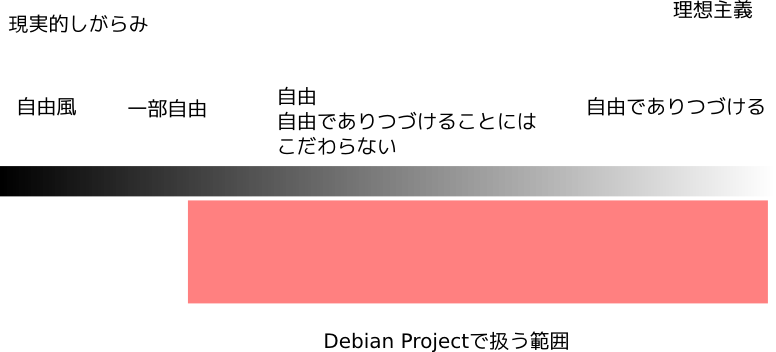
\includegraphics[width=1.1\hsize]{image200803/freerange.png}
\end{frame}

\begin{frame}{大雑把に自由なライセンスの類型でわけてみる}
\begin{itemize}
 \item 自由なものを自由でありつづけさせたいライセンス(GPLなど)
 \item 自由なものを不自由にする自由も与えたいライセンス(MIT, BSDなど)
 \item 自分の作ったものは自由につかってくれてよいが、自分の作成したもの
       は完全なため、勝手にいじってほしくない。よって、変更したものについて
       は明示的にしておいてほしいもの(LPPL 1.0など)
\end{itemize}
\end{frame}
\begin{frame}{Debian Projectでの使われ方}
\begin{itemize}
 \item Debian を有償・無償を問わず配布すること(DVD・公開ミラー・非公開
       ミラー)
 \item Debian を改変すること(Debianの改良、Debian外への流用、Debianから
       の派生ディストリビューションの開発など)
 \item Debianをあらゆる用途で利用できること(商用・教育用・宗教用・軍事
       用・医療用などを問わない)
\end{itemize}
\end{frame}

\begin{frame}{DFSG 1/2}

 {\scriptsize

     1. Free Redistribution

       The license of a Debian component may not restrict any party from
       selling or giving away the software as a component of an aggregate
       software distribution containing programs from several different
       sources. The license may not require a royalty or other fee for
       such sale.

    2. Source Code

       The program must include source code, and must allow distribution
       in source code as well as compiled form.

    3. Derived Works

       The license must allow modifications and derived works, and must
       allow them to be distributed under the same terms as the license
       of the original software.

    4. Integrity of The Author's Source Code

       The license may restrict source-code from being distributed in
       modified form {\bf only} if the license allows the distribution of
       "patch files" with the source code for the purpose of modifying
       the program at build time. The license must explicitly permit
       distribution of software built from modified source code. The
       license may require derived works to carry a different name or
       version number from the original software. (This is a compromise.
       The Debian group encourages all authors not to restrict any files,
       source or binary, from being modified.)

    5. No Discrimination Against Persons or Groups

       The license must not discriminate against any person or group of
       persons.

}
\end{frame}
\begin{frame}{DFSG 2/2}

{\scriptsize
    6. No Discrimination Against Fields of Endeavor

       The license must not restrict anyone from making use of the
       program in a specific field of endeavor. For example, it may not
       restrict the program from being used in a business, or from being
       used for genetic research.

    7. Distribution of License

       The rights attached to the program must apply to all to whom the
       program is redistributed without the need for execution of an
       additional license by those parties.

    8. License Must Not Be Specific to Debian

       The rights attached to the program must not depend on the
       program's being part of a Debian system. If the program is
       extracted from Debian and used or distributed without Debian but
       otherwise within the terms of the program's license, all parties
       to whom the program is redistributed should have the same rights
       as those that are granted in conjunction with the Debian system.

    9. License Must Not Contaminate Other Software

       The license must not place restrictions on other software that is
       distributed along with the licensed software. For example, the
       license must not insist that all other programs distributed on the
       same medium must be free software.

   10. Example Licenses

       The "GPL", "BSD", and "Artistic" licenses are examples of licenses
       that we consider "free".
 }
\end{frame}

\begin{frame}{Debian パッケージのライセンス管理}

発生するイベント
\begin{itemize}
 \item ITP
 \item New queue
 \item 再配布
 \item 改変
\end{itemize}
\end{frame}

\begin{frame}{debian/copyright}
\begin{itemize}
 \item README
 \item SOURCE
 \item BINARY
\end{itemize} 
\end{frame}



\section{}

\begin{frame}{宴会場所}

\begin{itemize}
 \item 宴会場所\\
       本日の宴会は「庵GuRi(あぐり) 5566」です。
       直前に人数を確定して 03-3780-5566 に電話してくださいと依頼されているので電話します。\\
       参加者はB1Fに集合し、全員で移動しましょう。
 \item 片付け\\
       部屋を片付けるのにご協力ください。
\end{itemize}

\end{frame}

\end{document}

;;; Local Variables: ***
;;; outline-regexp: "\\([ 	]*\\\\\\(documentstyle\\|documentclass\\|emtext\\|section\\|begin{frame}\\)\\*?[ 	]*[[{]\\|[]+\\)" ***
;;; End: ***
